\documentclass{article}


% if you need to pass options to natbib, use, e.g.:
%     \PassOptionsToPackage{numbers, compress}{natbib}
% before loading neurips_2023


% ready for submission
\usepackage[final]{neurips_2023}


% to compile a preprint version, e.g., for submission to arXiv, add add the
% [preprint] option:
%     \usepackage[preprint]{neurips_2023}


% to compile a camera-ready version, add the [final] option, e.g.:
%     \usepackage[final]{neurips_2023}


% to avoid loading the natbib package, add option nonatbib:
%    \usepackage[nonatbib]{neurips_2023}


\usepackage[utf8]{inputenc} % allow utf-8 input
\usepackage[T1]{fontenc}    % use 8-bit T1 fonts
\usepackage{hyperref}       % hyperlinks
\usepackage{url}            % simple URL typesetting
\usepackage{booktabs}       % professional-quality tables
\usepackage{amsfonts}       % blackboard math symbols
\usepackage{nicefrac}       % compact symbols for 1/2, etc.
\usepackage{microtype}      % microtypography
\usepackage{xcolor}         % colors
\usepackage{graphicx}       % for including images
\graphicspath{ {./images/} }

\title{CNN-based Ship Localization in Satellite Imagery: A U-Net Approach for the Airbus Ship Detection Challenge}


% The \author macro works with any number of authors. There are two commands
% used to separate the names and addresses of multiple authors: \And and \AND.
%
% Using \And between authors leaves it to LaTeX to determine where to break the
% lines. Using \AND forces a line break at that point. So, if LaTeX puts 3 of 4
% authors names on the first line, and the last on the second line, try using
% \AND instead of \And before the third author name.


\author{%
  Palásti András \\
  Student at Budapest University of Technology and Economics \\
  \texttt{andras.palasti@edu.bme.hu} \\
  \And
  Kurcsi Norbert \\
  Student at Budapest University of Technology and Economics \\
  \texttt{norbert.kurcsi@edu.bme.hu} \\
  \And
  Wittmajer Dávid \\
  Student at Budapest University of Technology and Economics \\
  \texttt{david.wittmajer@edu.bme.hu} \\
}


\begin{document}


\maketitle


\begin{abstract}
  In the context of the Airbus Ship Detection Challenge, searching for ships
  on the seas is akin to finding a needle in a haystack. Our paper addresses 
  this challenge by using a U-Net image segmentation model that relies 
  solely on convolutional layers to rapidly and accurately localize ships in 
  satellite images. This approach holds promising potential for enhancing ship
  detection technology and advancing the field of satellite image analysis.
\end{abstract}


\section{Introduction}


We developed our model for the Airbus Ship Detection Challenge, tasked with
swiftly and accurately identifying ships in satellite imagery. The objective is
to facilitate enhanced monitoring of oceans amidst increasing maritime traffic,
allowing environmental organizations, insurers, and governmental authorities to
better oversee potential incidents such as accidents, pirate attacks, illicit drug
and cargo transportation, and illegal fishing. Airbus provides crucial maritime
observation services, emphasizing the need for precise and prompt information delivery
to enhance the efficiency of their clients. 

The primary challenge lies in detecting ships that are obscured by clouds, navigating
adverse weather conditions, or are exceptionally small. Moreover, identifying vessels within
harbors amid diverse structures and terrain poses an additional difficulty. This paper
outlines our innovative approach to address these challenges and contribute to advancing
maritime surveillance capabilities.


\section{Related work}


\textbf{Convolutional Neural Networks (CNNs) in Object Detection}
Recent advancements in object detection have been significantly influenced by Convolutional
Neural Networks (CNNs). Ren et al. (2015) introduced Faster R-CNN, a seminal work that
integrates region proposal networks with CNNs for efficient object detection, laying the
foundation for subsequent improvements in accuracy and speed [1].

\textbf{Semantic Segmentation with U-Net}
The U-Net architecture, proposed by Ronneberger et al. (2015), initially gained prominence
in the field of medical image segmentation. Its application has since expanded due to its
efficacy and simplicity. U-Net's encoder-decoder structure, characterized by contracting
and expanding pathways, has been widely adopted in diverse segmentation tasks [2].

\textbf{Fully Convolutional Networks (FCN)}
The work of Long, Shelhamer, and Darrell (2014) introduced Fully Convolutional Networks (FCN)
for semantic segmentation, marking a significant milestone in end-to-end pixelwise labeling. 
FCN has laid the foundation for subsequent developments in semantic segmentation, influencing
the design of numerous segmentation architectures [3].

\textbf{Instance Segmentation Evaluation}
The work of Dollar et al. (2014) on the COCO (Common Objects in Context) dataset has served as
a benchmark for evaluating instance segmentation algorithms. The dataset provides a diverse
set of images with detailed annotations, facilitating rigorous evaluation of segmentation performance [4].

\textbf{ImageNet Pre-trained Models}
Razavian et al. (2014) explored the effectiveness of leveraging pre-trained CNN models on ImageNet for
image classification tasks. The use of pre-trained models has shown promise in feature extraction for
various applications, including remote sensing and satellite image analysis [5].

These diverse approaches collectively contribute to the growing body of literature in image
segmentation, providing insights and methodologies that address different challenges in the field.


\section{Architecture}


\begin{figure}
  \centering
  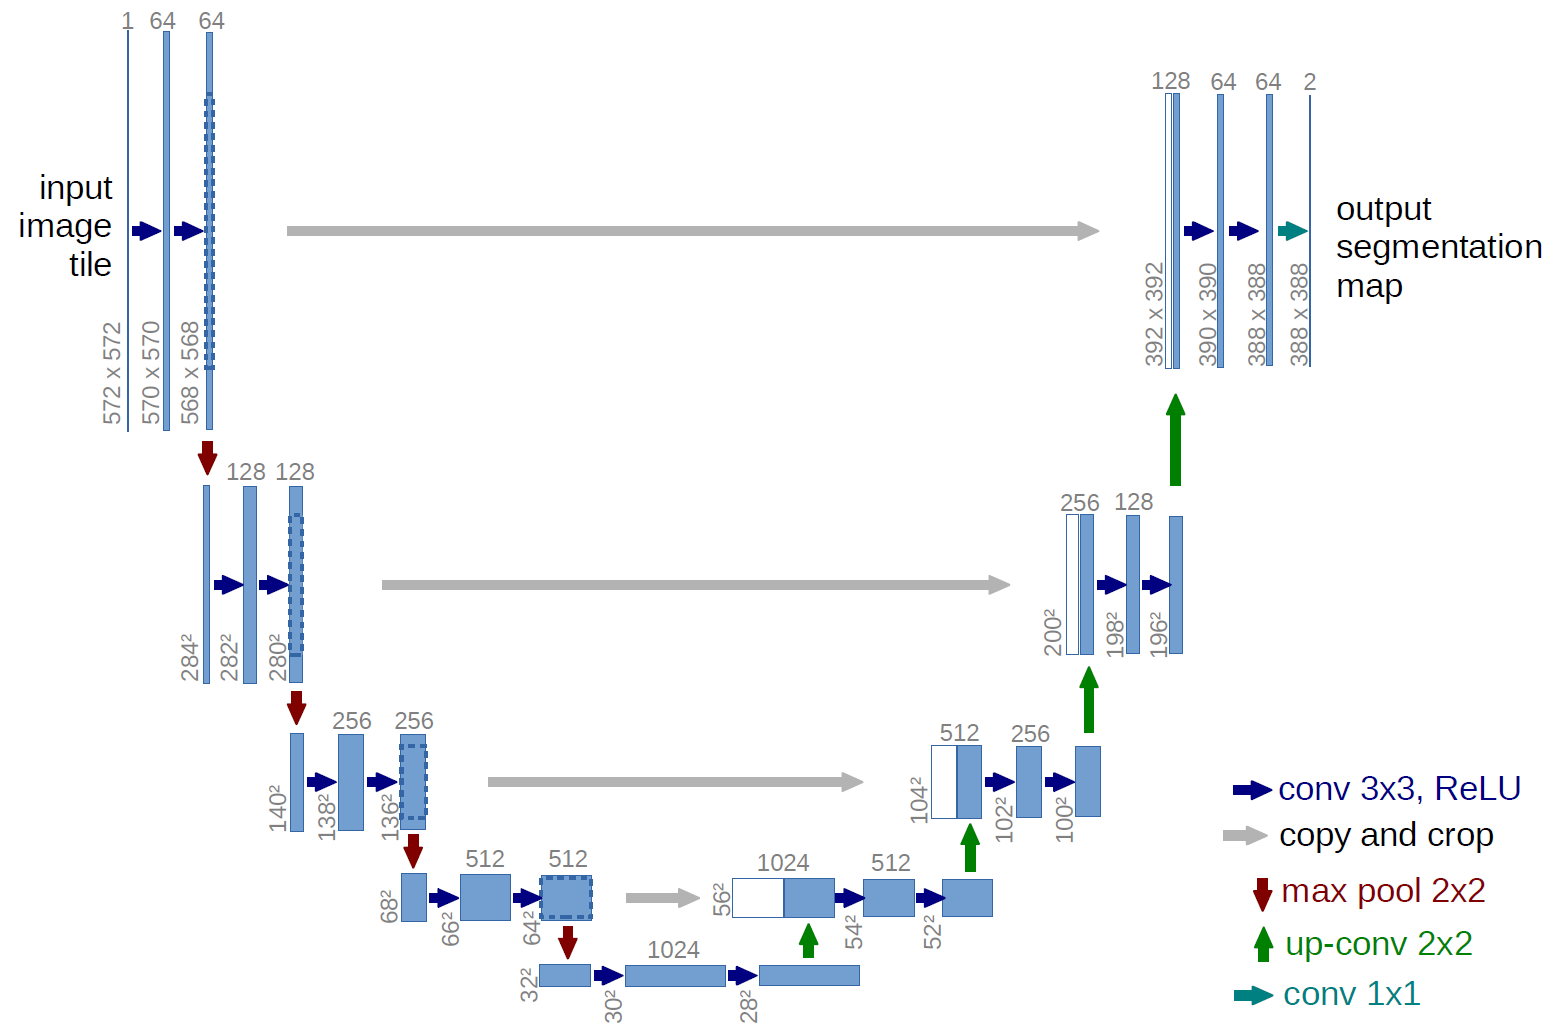
\includegraphics[width=0.8\textwidth]{u-net-architecture}
  \caption{
    The original UNet architecture was employed, albeit in a modified and simplified version.
    In this adaptation, the width and height of the input image tile align with the
    corresponding dimensions of the output segmentation.
  }
  \label{fig:unet}
\end{figure}


In our approach to the task, we employed a slightly modified UNet architecture, as depicted in Figure \ref{fig:unet}.
The sole deviation in our implementation lies in the absence of padding on the input image tile.
Consequently, the input size aligns with the dimensions of the output segmentation, specifically
matching in width and height. This was achieved by replacing the 'copy and crop' operations in
the original model. Instead, we first padded the smaller image with zeros to match the size of the larger
image and subsequently concatenated the two.


\section{Implementation}


\subsection{Data preparation}


Originally, the Airbus Ship Detection dataset comprised \(192556\) images. Out of these, only \(42556\) images contained
ships, accounting for less than 25\% of the dataset. Given the enormity of the full dataset for our specific requirements, 
and considering that the majority of images did not feature ships, we opted to utilize a subset of \(60000\) images. This
subset included all images containing ships (\(42556\) images) and additional images without ships (\(60000 - 42556 = 17444\) images).

We divided these images into training, validation, and test sets with ratios of 90\%, 5\%, and 5\%, respectively.
Our dataset is publicly available at the following URL: \url{https://drive.google.com/uc?id=1V-oxFZhctefBXL4noEgNG-ENaHoszTJE}.


\subsection{Training}


\begin{figure}
  \centering
  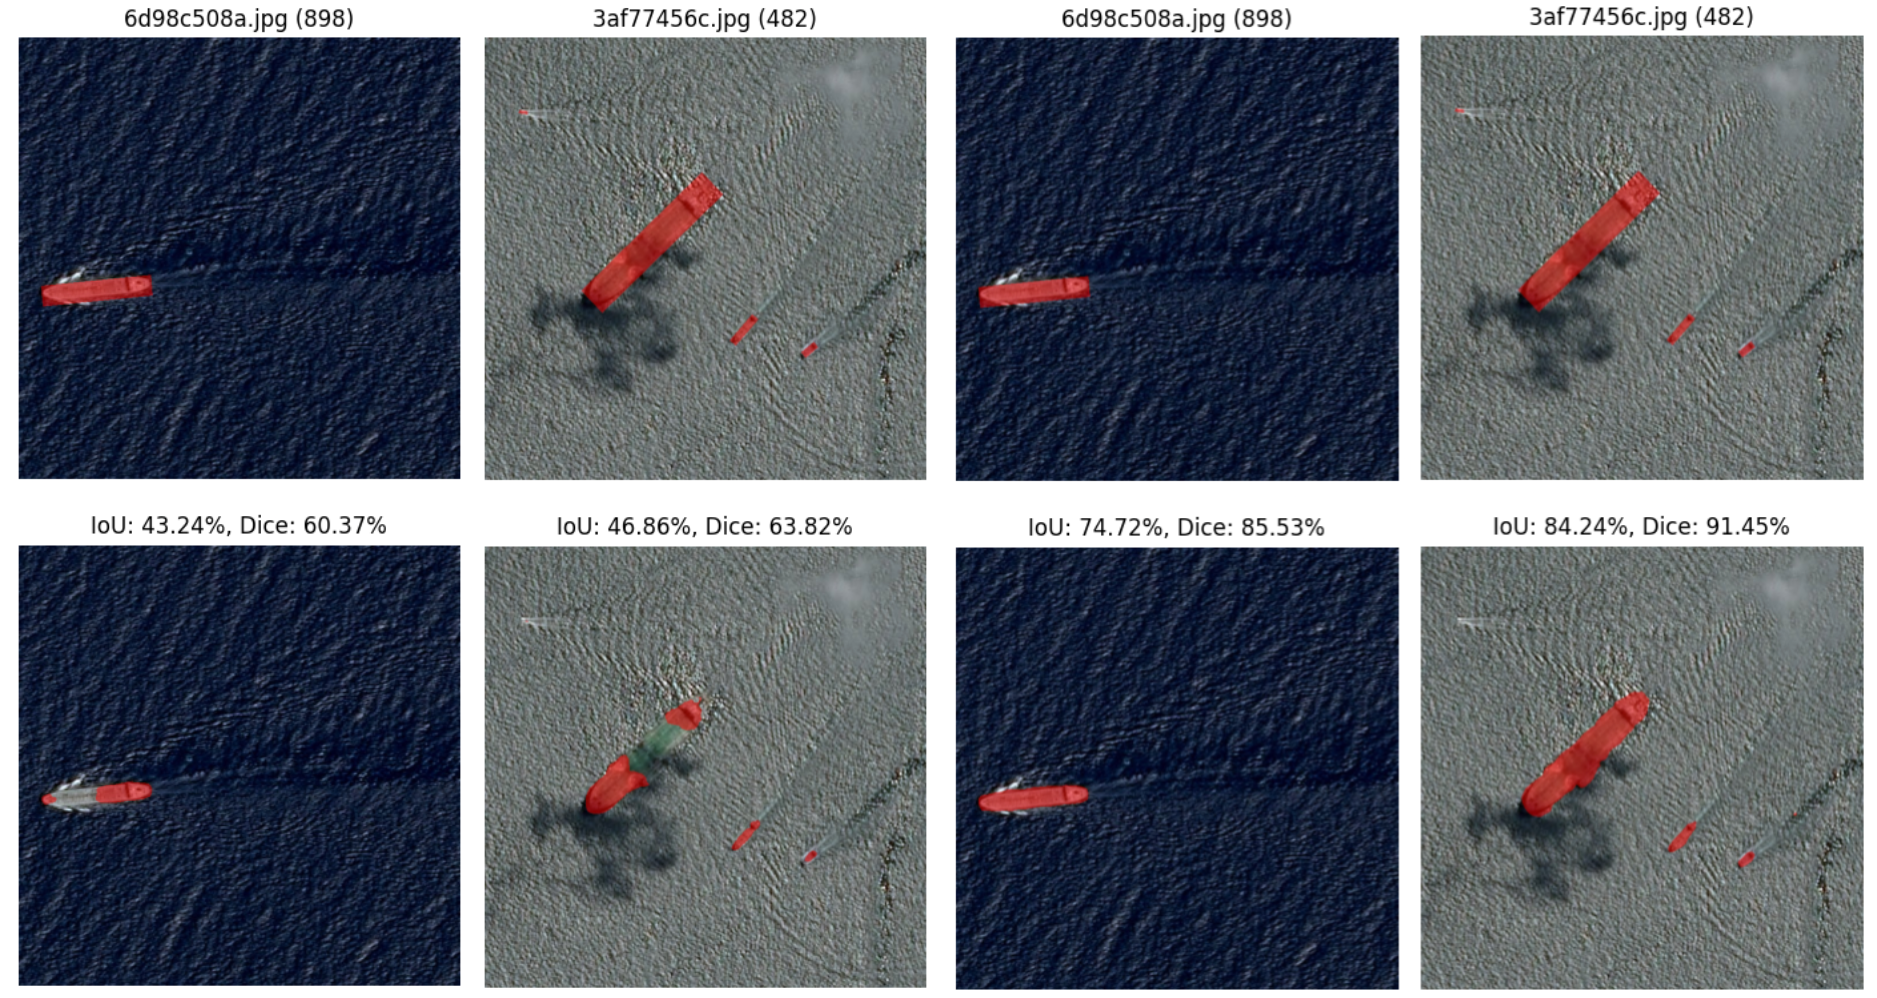
\includegraphics[width=\textwidth]{comparison}
  \caption{
    The top row depicts ground truth
    segmentations, and the bottom row shows predicted masks. The left side of the
    images corresponds to segmentations produced by a network trained on full-sized
    images, while the right side displays predictions from a network trained
    on cropped images.
  }
\end{figure}

For our initial solution, we employed the UNet model as described without engaging in intricate procedures.
The model was trained using provided training images and corresponding segmentation masks, with input
images sized \(768 \times 768\). The outcomes of this model are illustrated in Figure 2.

Our conjecture regarding the model's performance is that, when trained on full-sized images, it struggles
to discern crucial features due to the expansive context.

To address this issue, during training, we adopted a strategy of cropping a \(256 \times 256\) region from
the original training set image. If the image contains a ship, that region retains the ship; otherwise, a random
portion of the image is cropped. This approach ensures that our model receives training data in a more focused manner.


\subsection{Evaluation}

For our network's evaluation strategy, we considered two options: either performing predictions on the full-sized image
or splitting the image into \(256 \times 256\) parts and conducting predictions on each part. We experimented with both
approaches, and the results are presented in Table \ref{results-table}.

\begin{table}
  \caption{Results}
  \label{results-table}
  \centering
  \begin{tabular}{lll}
    \toprule
    Inference on             & IoU Score & Dice Score \\[0.1cm]
    \midrule
    Full-sized images        & $63.34\%$ & $72.88\%$  \\[0.1cm]
    $256 \times 256$ regions & $86.09\%$ & $87.90\%$  \\[0.1cm]
    $256 \times 256$ regions 
      that contain ships     & $60.68\%$ & $69.39\%$  \\[0.1cm]
    Full-sized images with 
      model trained on full 
      sized images           & $54.54\%$ & $63.39\%$  \\[0.1cm]
    \bottomrule
  \end{tabular}
\end{table}

As evident from Table \ref{results-table}, it may appear that our optimal strategy involves dividing the image into
\(256 \times 256\) regions and conducting inference on each region. However, this observation is misleading because
our evaluation includes images that do not contain any ships. Many of these ship-absent images achieve a perfect score
of \(1.0\), thereby inflating the mean of the scores. This is further substantiated by the fact that our results exhibit
a significant decline when we exclusively perform predictions on images containing ships.


\section{Conclusion}


In conclusion, our research highlights the crucial impact of training strategies on the performance of image segmentation
models. Through experimentation with different training methodologies, we observed a significant improvement in results when
the model was exposed to the most relevant portions of the data.

This approach proved to be particularly effective, leading to enhanced segmentation performance. The emphasis on training the model
with images containing ships, and carefully adjusting the segmentation masks accordingly, resulted in superior inference outcomes.


\section{Future improvements}


\begin{figure}[!hb]
  \centering
  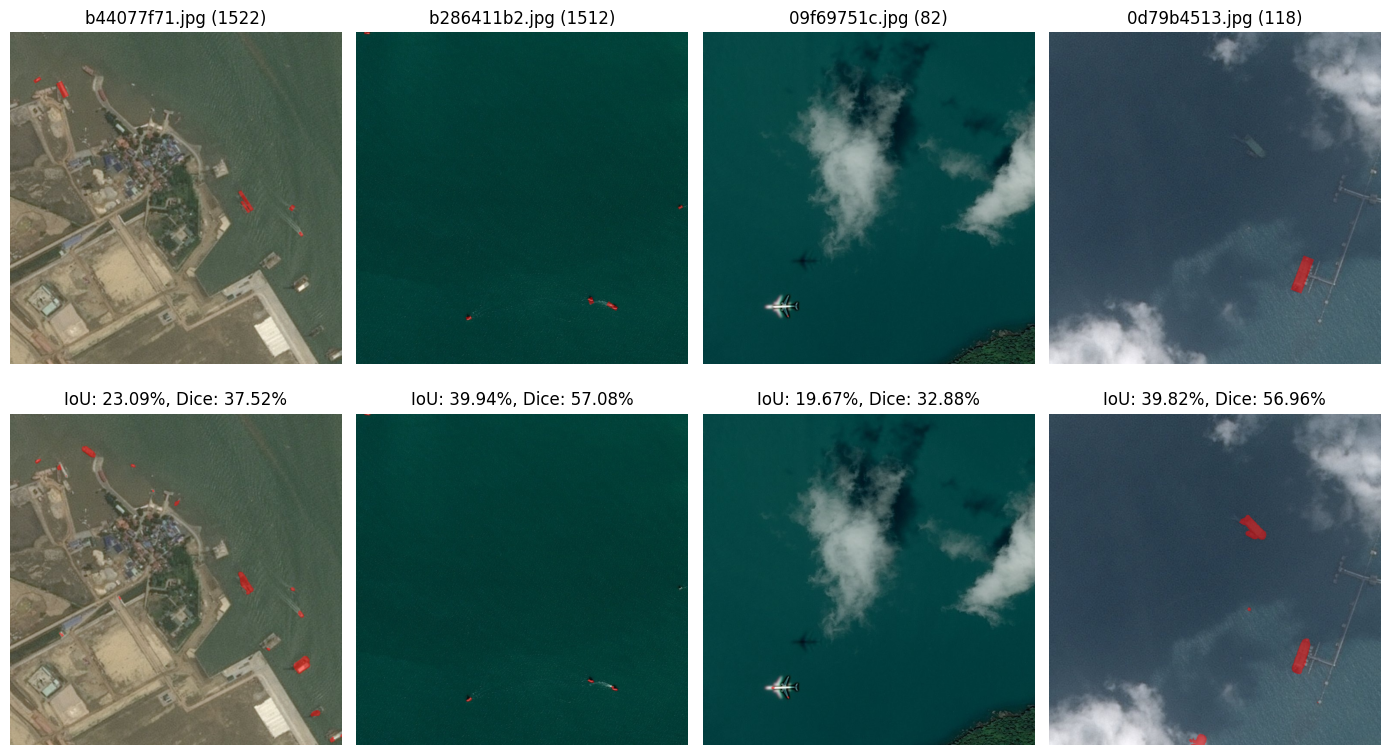
\includegraphics[width=\textwidth]{bad-segmentations}
  \caption{
    Some of the images where our model fail's to achive,
    respectable results.
  }
  \label{fig:bad-segmentations}
\end{figure}

While our current model demonstrates promising results, there are areas where improvements could significantly enhance its
performance. A careful examination of the worst segmentations, as depicted in Figure \ref{fig:bad-segmentations}, reveals
challenges in scenarios where land is present. Additionally, the model tends to struggle in distinguishing between
harbors and ships.

To address these weaknesses, a potential avenue for improvement involves a two-step training approach. Initially, training
on cropped images could allow the model to focus on learning the intricate details relevant to ship detection. Subsequently,
fine-tuning the model on full-sized images may help it generalize better to diverse scenes, including those with land and harbor
complexities.

This sequential training strategy aims to leverage the advantages of both cropped and full-sized images, allowing the model
to capture intricate details while maintaining a broader understanding of the overall context.


\section*{References}


\medskip
{
\small

[1] Ren, S., He, K., Girshick, R., \& Sun, J. (2015). Faster R-CNN: Towards Real-Time Object
Detection with Region Proposal Networks. In Advances in neural information processing
systems (pp. 91-99).


[2] Ronneberger, O., Fischer, P., \& Brox, T. (2015). U-Net: Convolutional Networks for
Biomedical Image Segmentation. In International Conference on Medical image computing and
computer-assisted intervention (pp. 234-241).


[3] Long, J., Shelhamer, E., \& Darrell, T. (2015). Fully Convolutional Networks for Semantic
Segmentation. In Proceedings of the IEEE Conference on Computer Vision and Pattern Recognition
(pp. 3431-3440).


[4] Dollar, P., Wojek, C., Schiele, B., \& Perona, P. (2012). Pedestrian Detection: An Evaluation
of the State of the Art. Pattern Analysis and Machine Intelligence, IEEE Transactions on, 34(4), 743-761.


[5] Razavian, A. S., Azizpour, H., Sullivan, J., \& Carlsson, S. (2014). CNN Features off-the-shelf:
an Astounding Baseline for Recognition. In Proceedings of the IEEE Conference on Computer Vision
and Pattern Recognition Workshops (pp. 806-813).
}


\end{document}